\documentclass[pdftex,11pt,a4paper]{article}
\usepackage{blindtext}
\usepackage{graphicx}
\usepackage{subfiles}
\usepackage{amsmath}
\usepackage{amsthm}
\usepackage{tikz}
\usepackage{wrapfig}
\usepackage{lscape}
\usepackage{rotating}
\usepackage{epstopdf}
\usepackage{subcaption}
\usepackage[font=small,labelfont=bf]{caption}
\usepackage{hyperref}
\usepackage{color}
\usepackage{algorithm}% http://ctan.org/pkg/algorithms
\usepackage{algpseudocode}% http://ctan.org/pkg/algorithmicx
\hypersetup{
    colorlinks=true,
    linkcolor=blue,
    citecolor=blue
}
\theoremstyle{definition}
\newtheorem{definition}{Definition}[section]
\newtheorem{theorem}{Theorem}[section]
\newtheorem{lemma}[theorem]{Lemma}
\theoremstyle{remark}
\newtheorem*{remark}{Remark}
\usepackage{amssymb}
\usepackage{amsfonts}
\usepackage{mathtools}
\usepackage{geometry}
 \geometry{
 a4paper,
 total={210mm,297mm},
 left=30mm,
 right=30mm,
 top=30mm,
 bottom=35mm,
 }
\newcommand{\defeq}{\vcentcolon=}
\newcommand{\eqdef}{=\vcentcolon}
\newcommand*{\V}[1]{\mathbf{#1}}%
\newcommand{\norm}[1]{\left\lVert#1\right\rVert}
\newcommand{\justif}[2]{&{#1}&\text{#2}}
\newcommand{\qedwhite}{\hfill \ensuremath{\Box}}
\newcommand\given[1][]{\:#1\vert\:}
\newcommand{\me}{\mathrm{e}}
\DeclarePairedDelimiterX{\infdivx}[2]{(}{)}{%
  #1\;\delimsize\|\;#2%
}
\DeclarePairedDelimiter\abs{\lvert}{\rvert}%
\newcommand{\Conv}{\mathop{\scalebox{1.5}{\raisebox{-0.2ex}{$\ast$}}}}%
\newcommand{\infdiv}{\infdivx}
\newcommand\tab[1][1cm]{\hspace*{#1}}
\newcommand{\parder}[2]{\frac{\partial{#1}}{\partial{#2}}}
\renewcommand{\qed}{\hfill\blacksquare}
\hyphenation{op-tical net-works semi-conduc-tor tech-no-lo-gy}
\title{A succinct introduction to LSTMs}
\author{Bernardo P\'erez Orozco}
\date{July 2016}

\begin{document}

\maketitle

\section{Introduction}
In these notes, we will outline some recent developments in Machine Learning that entail mostly the Long Short Term Memory (LSTM) architecture and the gradient descent optimisation method. In order to fully understand the contribution made by LSTMs, it is necessary to build a historical path developing on how they came to existence.

\par In particular, LSTMs are a special case of the more general Recurrent Neural Networks (RNNs). RNNs have been known to be difficult to train by means of gradient descent methods because they suffer from the vanishing gradient problem, which prevents them from learning long term dependencies. The LSTM architecture directly tackles this problem by incorporating a gating mechanism that allows training error signals to flow backwards for long periods of time, and hence is able to learn long term relations using gradient-based methods.

\par This document is structured as follows: in Section \ref{sec_path} we give a refresher on basic Neural Networks concepts, summarise recent upgrades developed for gradient descent methods, and discuss the RNN architecture and the vanishing gradient problem. In Section \ref{sec_lstm} we introduce the LSTM architecture and show how they solve the vanishing gradient problem. Then, in Section \ref{sec_keras} we introduce the Keras framework and show how it can be used for swift development of deep learning applications. Finally, in Section \ref{sub_future}, we give an account of further thoughts for future work and opportunities for LSTMs in both the research community and industry.

\section{A review of Neural Networks} \label{sec_path}
In this section, we give a brief refresher of basic concepts of neural networks. Throughout this tutorial, we will present several architectures that should be thought of as blocks. Connecting these blocks or layers using a specific topology yields what we traditionally call \textit{a neural network}. 

\par A neural network layer contains computing units, also called \textbf{neurons}. Each neuron receives a vector input $\V{x}$ and computes a scalar $h$ called the \textbf{activation} of the neuron. The activation value computed by each individual unit describes the amount of activity in the neuron, and hence we can think of them as \textbf{feature detectors}, i.e. certain stimuli (features) will increase the activity of specific units. The vector of activations $\V{h}$ is obtained by gathering the activation values of all individual neurons in a single layer, and it describes the current state of the layer. This information can be used by other blocks in the network to make decisions, such as classifying the input or forecasting a time series.

\begin{figure}[t]
    \centering
    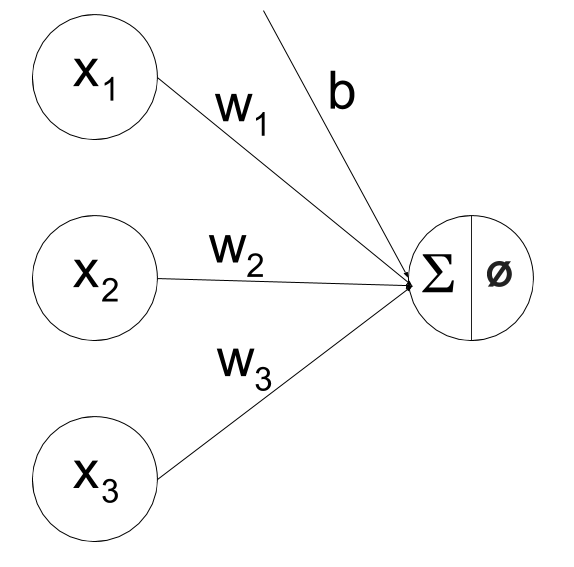
\includegraphics[width=5.5cm]{figs/neuron.png}
    \caption{The dense unit is fully connected to all units in the previous layer. Each edge is weighted by a scalar $w_i$, and the function learnt by the neuron has a vertical shift given by a bias $b$. The activation of the dense unit is given by $h = \phi(\V{w}^T\V{x} + b )$.}
    \label{fig:neuron} 
\end{figure} 

\par The simplest case of a neural network is called a Multilayer Perceptron (MLP) and comprises three layers: an input layer, a hidden layer, and an output layer. These are connected one after the other, i.e. in a feedforward fashion. The hidden and the output layers are both instances of \textbf{dense layers}. Each neuron in a dense layer is fully connected to all the neurons in the previous layer and its activation is given by $h = \phi(\V{w}^T\V{x} + b)$, where $\V{w}$ is the parameter vector of the neuron, $b$ is the bias parameter of the layer, $\V{x}$ is the input to the layer, and $\phi$ is called the activation function, as seen in Figure \ref{fig:neuron}.

\par However, neural networks are generally thought of in terms of layers, and not individual neurons. We can think of layers more generally as mappings (characterised by some fixed parameters $\theta$) between two spaces, and then a neural network is created by connecting them (as seen in Figure \ref{fig:mlp}). For example, we can think of dense layers as mappings $H:\mathbb{R}^n \rightarrow \mathbb{R}^m$ given by $H(\V{x}) = \phi(\V{Wx}+\V{b})$, where:

\begin{figure}
    \centering
    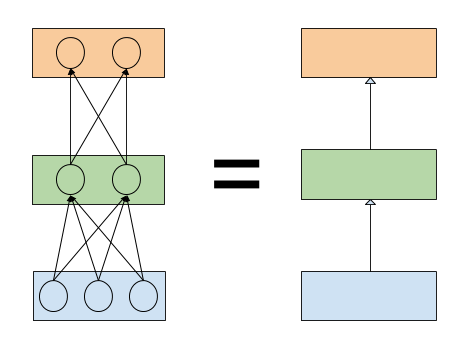
\includegraphics[width=6cm]{figs/mlp.png}
    \caption{Although the processing units of neural networks are its hidden units, the model itself can be thought of as a set of interconnected layers. Each layer can be thought of as a mapping with a specific shape.}
    \label{fig:mlp}
\end{figure}

\begin{itemize}
    \item The entries of the output vector $\V{h} = H(\V{x})$ are called the \textit{activations} of the layer.
    \item $\phi$ is an element-wise function called the \textit{activation function}.
    \item $m$ is called the \textit{size} of the layer, and refers to the number of \textit{hidden neurons} it has.
    \item $\V{W, b}$ are called the parameters of the layer.
\end{itemize}

\par Activation functions are often called \textit{non-linearities}, since they are expected to be non-linear - some common examples in the literature are the sigmoid activation function, the hyperbolic tangent and the rectified linear unit, given respectively by:
\begin{align*}
    \sigma(x) &= \frac{1}{1+e^{-x}}\\
    \text{tanh}(x) &= \frac{e^x - e^{-x}}{e^x + e^{-x}}\\
    \text{ReLU}(x) &= \max(0, x)
\end{align*}

\par Remark that the usage of non-linearities is crucial for allowing neural networks to learn complex relations in data. Each successive layer will receive as input a vector that will have gone through a non-linear transformation, and therefore neural networks are able to learn very complex, non-linear geometries.

\par It can be shown that an MLP with one hidden layer with a linear activation function can be reduced to an MLP with only an output layer, and therefore linear activations are reserved for output layers in regression problems, i.e. when we are concerned with unconstrained, continuous output.

\par Recent developments in the field have seen the introduction of several other types of layers, such as the convolutional layer, the autoencoder and the LSTM cell - all of which have played a key role in the ``deep learning revolution''. In this work, we are mainly concerned with the LSTM cell architecture, which will be introduced alongside its applications and shortcomings in the next sections.

\subsection{Deep Learning}

\par We are now prepared to discuss a number of questions that arise in the study of neural networks:

\begin{itemize}
    \item How many and what type of layers should the network have?
    \item How many hidden units should each layer have?
    \item What activation function should each layer have?
    \item Given a problem, how do we find the parameters for each layer that give the best solution?
\end{itemize}

\par It is now worth saying that none of the questions above has a clear answer, and they still represent a priority in the neural network agenda. As of this date, a great portion of the serious scrutiny of the deep learning wave concerns the black-box nature of neural networks. Despite the empirical success in areas such as image recognition, speech recognition, machine translation, etc. the academic community still has many open questions in addition to the above, e.g. is the hidden representation learnt by intermediate layers meaningful in any way? Is there a mathematical relation between the data and the optimal number of parameters (i.e. topology of the network)? 

\par As a consequence, there is no clear consensus on the definition of ``deep learning'', and thus is often only taken to mean the use of layered models (such as neural networks) with a \textit{greater} number of modules than the state of the art a few years ago. Therefore, some members of the academic community might consider a 5-layer model to be a deep one, although a large portion of the most successful state-of-the-art models will actually have more than 10 \cite{Szegedy,Simonyan2015}.

\par Before the deep learning wave, MLPs had been proven to be universal approximators by Cybenko \cite{Cybenko1993}. However, the proof does not state any theoretical guarantees about the number of hidden units required for this architecture to learn an arbitrary concept - which may even turn out to be exponential. Moreover, this approach required the development of handcrafted data feature extraction techniques. 

\par Therefore, one motivation for using deeper architectures concerned automatically learning features in a hierarchical fashion, i.e. assuming that a a sequential application of linear and non-linear transformations would output an optimal feature representation from data, and that an additional dense layer could be used to perform the desired task (regression, classification, etc.). However, the lack of specialised hardware and software in the 80s and 90s disabled the academic community from bringing these models to life. This is one of the main reasons why, even though it was actually conceived last century, it is only now that we have seen deep learning in practice.

\par One of the most successful deep learning models is the Long Short Term Memory (LSTM) cell, which are a recurrent architecture that enables efficient learning of vanilla Recurrent Neural Networks (RNNs). In the next subsections, we introduce recurrent networks and training by gradient descent, which naturally leads to a presentation of the LSTM architecture.


\subsection{Recent developments for gradient descent}

Given a sequence of layers $H^{(1)}, H^{(2)}, ..., H^{(L-1)}$, where $L$ is the number of modules in the network, we are now concerned with finding the values of each layer's parameters, e.g. if $H^{(i)}$ is a dense layer, we now want to find the values of $\V{W^{(i)}, b^{(i)}}$ that optimise a \textit{criterion}, also called a \textit{loss function}. The criterion is chosen with respect to the sort of problem to be tackled, and is parametrised by the data's ground truth, for example:

\begin{itemize}
    \item \textbf{Minimum squared error}. Defined as the 2-norm distance between the predictions and the ground truth: $L_\text{MSE}(\hat{\V{y}}) = \norm{\V{\hat{y}} - \V{y}}^2$. This is a common choice for regression problems.
    \item \textbf{Cross-entropy}. Tihs can be used as a measure of the error between two probability distributions, namely a target distribution and a learnt distribution. Classification problems can also be reformulated as learning probability distributions, and hence this loss function is often used in such problems.
    \item \textbf{Hinge loss}. In classification problems, this margin-based function increases based on the number of misclassifications produced by the algorithm. For the binary case with ground truth and prediction $\hat{y}, y\in\{1, -1\}$, the hinge loss is given by $L_\text{hinge}(\hat{y}) = \max{(0, 1 - \hat{y} \odot y )}$.
\end{itemize}

%cite: http://www.cs.toronto.edu/~graves/icml_2006.pdf
\par The loss function speaks about the fitness of our predictions with respect to the data. This is why tailored loss functions may be in place depending on the problem; for example, multiclass loss functions do exist for classification problems with more than one category; another example is the Connectionist Temporal Classification loss \cite{Graves2013}, which improves sequence classification by ``removing inherently ambiguous label boundaries and allowing label predictions to be grouped together if it proves useful''.

\par Once the loss function has been chosen, we can use an optimisation method to minimise it. The most widespread method in the neural network community is gradient descent, which finds an optimal solution in an iterative fashion. However, it is worth noting that many alternatives are still being researched, for example evolutionary algorithms \cite{Sexton1999,Schmidhuber2007}, Bayesian optimisation techniques \cite{DeFreitas1999} and Kalman filters \cite{Tobergte2013}.

\par Gradient descent has been the method of choice by most in the community due to its simplicity, but also because its main disadvantage (getting stuck in local minima) does not have a major empirical impact in most scenarios, since local minima solutions generally offer state-of-the-art results already.

\par The vanilla version of gradient descent updates the parameters $\theta$ once per epoch (a single scan of the dataset) using the rule:
\begin{align*}
    \theta_{t+1} = \theta_{t} - \alpha \nabla_\theta L(\theta) 
\end{align*}

where $\alpha$ is called the learning rate and $L$ is the loss function to minimise. Recent developments to this vanilla version of gradient descent (and which have seen the light of day on par with the deep learning wave) include:

\begin{itemize}
    \item The advent of big datasets has made a single computation of the true gradient of $L$ too expensive, since a single update operation requires a scan of the whole dataset. \textbf{Minibatch stochastic gradient descent} (minibatch SGD) \cite{Bottou2010} instead computes an approximation of the gradient using only a (random) ``minibatch'' of the dataset. The approximate gradient is computed as the empirical mean of the gradient evaluated at each individual data point in the dataset. As the number of points used to take the empirical mean grows larger, we expect the approximation to converge to the true gradient. This variant of gradient descent is stochastic because the approximate gradient is a random variable subject to the random minibatch - this helps the method escape from local minima if it gets stuck, and also encourages the exploration of a larger area of the loss function (as opposed to the deterministic nature of vanilla gradient descent, which always explores the same area for the same given initial conditions).
    \item The value of the learning rate $\alpha$ hyperparameter can greatly influence the performance of the algorithm. A value too large and the algorithm will struggle to converge. A value too small and the algorithm will take a very long time to finish. Furthermore, some input features may be sparser than others, and thus we would like to take full advantage of their rare occurrences. \textbf{Adaptive Learning Rate} methods aim to solve both of these issues by allowing the learning rate to adapt automatically over time, normally considering information unveiled by previous gradient computations. AdaGrad (Adaptive Gradient) \cite{Duchi2011} was the pioneer in this class of techniques. Let $g_\tau$ be the approximate gradient at time $\tau$, and let $G_i=\sum_{\tau=1}^t g_{\tau, i}^2$. Then the update for the i-th parameter $\theta_i$, using a smoothing factor $\epsilon$ and initial learning rate $\alpha$, is given by:
    \begin{align*}
        \theta_{t+1, i} = \theta_{t, i} - \frac{\alpha}{\sqrt{G_i + \epsilon}}g_{t, i}
    \end{align*}
    \item The descent can gain \textbf{momentum} by allowing new updates to consider previous updates \cite{Ruder2015}, i.e. if $\theta_{t+1} = \theta_t - \nu_t$, then allow $\nu_t = \gamma\nu_{t-1} + \alpha\nabla_\theta L(\theta)$, where $\gamma$ is called the momentum factor. Therefore the updates are always pulled or corrected by our knowledge of previous gradients. This greatly dampens the effect of very noisy approximations to the true gradient, while also encouraging taking steps in the best direction.
    
\end{itemize}

%http://sebastianruder.com/optimizing-gradient-descent/index.html#stochasticgradientdescent
\par Some recently developed algorithms that implement these improvements are Adadelta, RMSprop and Adam. Although they all have a similar performance \cite{Kingma2014}, Adam is the one that has shown the best empirical results so far. Adam stands for Adaptive Moment Estimation, where moment in this case refers to the bias-corrected estimates of the first- and second-order moments of the gradient. Adam keeps an exponentially decaying sum of gradients that emulates the performance of momentum. The update equations are given below:

\begin{align*}
    \theta_{t+1} &= \theta_t - \frac{\alpha}{\sqrt{\hat{v_t}} + \epsilon}\hat{m_t}\\
    \hat{m_t} &= \frac{1}{1 - \beta_1^t}\beta_1 m_t\\
    \hat{v_t} &= \frac{1}{1 - \beta_2^t}\beta_2 v_t\\
    m_t &= \beta_1m_{t-1} + (1 - \beta_1)g_t\\
    v_t &= \beta_2v_{t-1} + (1 - \beta_2)g_t^2
\end{align*}

\par One key point we have not discussed in the gradient descent presentation (no matter what flavour is to be used) is the computation of the gradient itself. Traditionally, neural networks have benefited from an algorithm backpropagation, which is an efficient way of computing the gradient $\nabla_\theta L(\theta)$. Backpropagation is neither numeric (finite differences) nor symbolic differentiation. 

\par Instead, one could claim that backpropagation is ``a clever way'' of taking advantage of the chain rule and the graph structure of the neural network so as to compute derivatives efficiently. It turns out that backpropagation is in reality a special case of \textbf{automatic differentiation} (AD), which is a general method to compute derivatives of computer programs \cite{Kingma2014}. In other words, if we have a program $P$ that computes a function $f(\V{x})$, and we are interested in taking its gradient $\nabla_\V{x}f$, then we can represent the program as a computational graph (which we already did in neural networks!) that can be traversed. This traversal is equivalent to a successive application of the chain rule to each statement in the program $P$, and it generates a new program $P'$ that computes the gradient $\nabla_\V{x} f(\V{x})$.

\par Crucially, AD is fundamentally different from numerical and symbolic differentiation, and introduces several advantages with respect to them: it does not introduce round-off or approximation errors, unlike finite differences; in addition, AD returns an efficient way of computing the gradient, unlike symbolic differentiation, which requires additional computational power to perform all appropriate simplifications; finally, AD takes full advantage of intermediate results to compute the derivative of a vector function with respect to each of its inputs efficiently - both numerical and symbolic differentiation require an independent run to take the derivative of the function with respect to each input. More details of the AD framework can be found in \cite{Bucker2005ADA}.

\par AD has further enhanced the interest in the development of gradient descent methods. In fact, it is now a key component in most (if not all) specialised software frameworks for deep learning. Importantly, the frameworks Theano, Torch and Tensorflow implement AD. This has enabled all three frameworks to develop a maintainable design in which new activation and loss functions can be incorporated with little effort.

\subsection{Recurrent Neural Networks}
The networks we have discussed so far have comprised layers connected one after the other, i.e. in a feedforward fashion. We now turn our attention to networks that are allowed to form a cyclical topology. These models are called \textbf{Recurrent Neural Networks} (RNNs).

\par The simplest case, and the one we will be discussing for the rest of this document, concerns layers that have a connection to themselves, i.e. $\V{h}_t = f(\V{h}_{t-1}, \V{x}_t ; \theta)$, where $\V{x}_t$ is the input to the layer at time $t$. This equations is the standard equation of a dynamical system. We can see this relation more clearly by unrolling the network as seen in Figure \ref{fig:rnn}. This means that this architecture enables us to train models over sequences.

\begin{figure}[t]
    \centering
    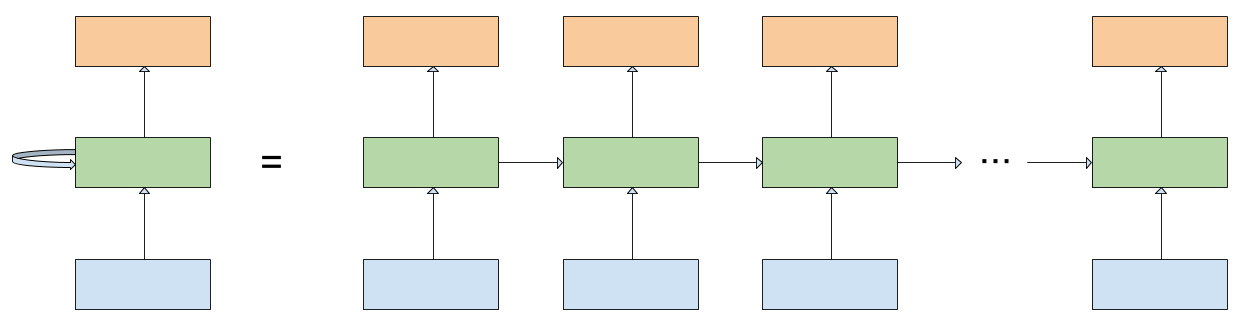
\includegraphics[width=\textwidth]{figs/rnn.png}
    \caption{Recurrent neural networks have at least one directed cycle, often present in the form of a self-connected layer. The resulting graph and be unfolded as a grid, which enables sequence learning to be visualised more clearly.}
    \label{fig:rnn}
\end{figure}

\par The \textbf{RNN layer} is the extension of the dense layer for the recurrent topology, and is given by:
\begin{align*}
    \V{h}_t = \phi(\V{W_rh}_{t-1} + \V{W_ix}_t + \V{b})
\end{align*}

\par i.e. we now have an extra matrix of parameters in comparison with the dense layer. For convenience, we can also define it in the following way:
\begin{align*}
    \V{h}_t = \V{W_r}\phi(\V{h_{t-1}}) + \V{W_ix}_t + \V{b}
\end{align*}

%CITE: http://www.jmlr.org/proceedings/papers/v28/pascanu13.pdf
\par From the equation above, it is easy to see that $\V{h}_t = f(\V{h}_{t-1}, \V{x}_t, \theta)$, and furthermore $\V{h}_t = f(f(...f(\V{h}_0, \V{x}_1, \theta)..., \V{x}_{t-1}, \theta), \V{x}_t, \theta)$, where $\V{h}_0$ is the initial state of the recurrent network. 
\par We are now interested in computing the derivatives of $\V{h}_t$ wrt $\theta$ so as to use gradient descent. A careful derivation of these is given in \cite{Pascanu2012}. However, we will briefly discuss the crucial term $\frac{\partial\V{h}_t}{\partial\theta_j}$, where $\theta_j$ is any parameter in $\theta$. Using the product rule and the chain rule, we can see that:
\begin{align*}
    \frac{\partial\V{h}_t}{\partial\theta_j} &= \frac{\partial\V{W}_r}{\partial\theta_j} \phi(\V{h_{t-1}}) + \V{W}_r\frac{\partial \phi(\V{h}_{t-1})}{\partial\V{h}_{t-1}}\frac{\partial \V{h}_{t-1}}{\partial\theta_j}\\
    &= \frac{\partial\V{W}_r}{\partial\theta_j} \phi(\V{h_{t-1}}) + \V{W}_r\phi'(\V{h}_{t-1})\frac{\partial \V{h}_{t-1}}{\partial\theta_j}\\
    &= \frac{\partial\V{W}_r}{\partial\theta_j} \phi(\V{h_{t-1}}) + \V{W}_r\phi'(\V{h}_{t-1})\left(\frac{\partial\V{W}_r}{\partial\theta_j} \phi(\V{h_{t-2}}) + \V{W}_r\phi'(\V{h}_{t-2})\frac{\partial \V{h}_{t-2}}{\partial\theta_j}\right)
\end{align*}
\par As we further expand the recursive terms, we can see that new terms will have a greater number of instances of the activation function. This can be troublesome, especially with common activation functions such as tanh and the sigmoid, since their derivatives are never greater than 1. This is the fundamental drawback of Recurrent Neural Networks: 
\begin{itemize}
    \item The increasing number of instances of the activation function will lead the gradient to \textbf{vanish}, i.e. terms that appear later in the recursion will tend to zero and the model will not be able to learn long term dependencies.
    \item If the activations are maintained close to 1, but the weights are considerably larger, then adding them up will lead to an \textbf{exploding gradient}. Similarly, this makes it extremely difficult or even impossible (if the gradient overflows the arithmetical precision) for gradient descent to converge.
\end{itemize}

\par In \cite{Pascanu2012}, the authors propose a \textbf{gradient clipping} method to avoid exploding gradients. The authors show how exploding gradient correspond to ``walls'' in the geometry of the loss function. Following the gradient in this case makes the algorithm take a large step away from the wall, and possibly miss the information of the region that lies close by. Instead, the gradient can scaled down whenever it explodes, so as to make the algorithm barely move away from the wall and keep exploring that region. 

\par The clipping rule is given by:
\begin{algorithm}
\begin{algorithmic}[1]
\Function{clip}{$L, \theta, \epsilon_{\text{clip}}$}
\State $\hat{\V{g}} \leftarrow \parder{L}{\theta}$
\If{$\norm{\hat{\V{g}}} \geq \epsilon_{\text{clip}}$}
\State $\norm{\hat{\V{g}}}\leftarrow \frac{\epsilon_{clip}}{\norm{\hat{\V{g}}}}\hat{\V{g}}$
\EndIf
\EndFunction
\end{algorithmic}
\end{algorithm}

\par Gradient clipping has shown good empirical results and has largely become a necesasry ingredient for training any sort of recurrent network. Although there were many attempts at finding how to overcome these difficulties, the most successful so far comprises fundamental changes in the recurrent layer. This resulted in the creation of the \textbf{LSTM layer}, which we are now prepared to discuss in the next Section.

\section{The LSTM architecture} \label{sec_lstm}

We now turn our attention to the LSTM architecture. In subsection \ref{sub_lstm}, we will introduce the LSTM cell and show how it solves the vanishing gradient problem. Then, in subsection \ref{sub_apps} we outline a reading list for LSTM applications. 

\subsection{The LSTM cell solves the vanishing gradient problem} \label{sub_lstm}
The LSTM layer \cite{Gers2002,Hochreiter1997} directly addresses the issue of the vanishing gradient by means of a gating mechanism, and is given by the following equations:

\begin{align*}
    \V{x}'_t &= [ \V{x}_t, \V{h}_{t-1} ]\\
    \V{S}_t &= \tanh(\V{W}_S\V{x}'_t + \V{b}_S)\\
    \V{C}_t &= \V{i}_t\odot\V{S}_t + \V{f}_t\odot\V{C}_{t-1}\\
    \V{h}_t &= \V{o}_t \odot \tanh(\V{C}_t)
\end{align*}
\par where $\V{i}_t, \V{o}_t, \V{f}_t$ are called the input, output and forget gates respectively, and are given by:
\begin{align*}
    \V{i}_t &= \sigma(\V{W}_i\V{x}'_t + \V{b}_i)\\
    \V{o}_t &= \sigma(\V{W}_o\V{x}'_t + \V{b}_o)\\
    \V{f}_t &= \sigma(\V{W}_f\V{x}'_t + \V{b}_f)
\end{align*}

\par We call $\V{C}_t$ the \textit{memory cell} at time $t$, and it is arguably the main component of the LSTM architecture. It simulates a computer READ and WRITE operations over its memory. For example, we can think of the memory cell equation given above as follows:

\begin{align*}
    \V{C}_t &= \V{i}_t\odot\V{S}_t + \V{f}_t\odot\V{C}_{t-1}\\
    \text{memory}_t &= \text{read}\odot\text{input}_t + \text{remember}\odot\text{memory}_{t-1}
\end{align*}

\par Crucially, the LSTM architecture is based on a \textbf{Constant Error Carousel} (CEC). When thinking of the network as an unfolded computational graph, backpropagation allows the error signal to flow backwards across the nodes. However, a vanishing gradient architecture will dampen the signal as it traverses the graph by a factor given by the derivatives of the activation function. 

\par In other words, we need to stabilise the products $\V{W}_r\phi'{(\V{h})}$ by making them approach $\V{1}$. One way to do this is to regularise the weights while also using a linear activation function for the recurrent edges.  The LSTM layer manages to address this by introducing specialised gates that control the state of each memory cell by regulating the influx of its two main sources: the input at time $t$ and the storage at time $t-1$. Importantly, the behaviour of the gates is also a learning target since we introduce new parameters $\V{W}_i, \V{W}_o, \V{W}_f$ correspondingly.  

\par Note that the memory cell $\V{C}_t$ is only squashed in the feedforward arrows of the networks, and remarkably not in the recurrent computations, i.e. $\V{C}_t$ is a function of $\V{C}_{t-1}$ without any activation. To observe this more formally, we can make a derivation similar to the one for the RNN layer:

\begin{align*}
    \parder{\V{h}_t}{\theta_j} &= \parder{\V{o}_t}{\theta_j}\odot \tanh(\V{C}_t) + \V{o}_t\odot\parder{\tanh(\V{C}_t)}{\V{C}_t}\parder{\V{C}_t}{\theta_j}\\
    \parder{\V{C}_t}{\theta_j} &= \parder{\V{i}_t}{\theta_j}\odot\V{S}_t +  \V{i}_t\odot\parder{\V{S}_t}{\theta_j} + \parder{\V{f}_t}{\theta_j}\odot\V{C}_{t-1} + \V{f}_t\odot\parder{\V{C}_{t-1}}{\theta_j}
\end{align*}

\par By using a similar reasoning to the previous derivation, we can see that the factors $\parder{\V{i}_t}{\theta_j}, \parder{\V{o}_t}{\theta_j}, \parder{\V{f}_t}{\theta_j}, \parder{\V{S}_t}{\theta_j}$ may all (partially) vanish, since they are recursive (dependent on $\V{x}'_t$) and have the shape $\phi(\V{Wx}'_t + \V{b})$. 

\par Nevertheless, the term $\parder{\V{C}_t}{\theta_j}$ is also a function of $\parder{\V{C}_{t-1}}{\theta_j}$, which is different in two ways: firstly, the recursive factor $\V{C}_{t-1}$ is not squashed by any activation function. Secondly, each recursive term is weighted by the element-wise product of the previous $k$ forget gates $\prod_{T=k}^t\V{f}_T$. Therefore, the gradient only vanishes for terms that contain $\V{f}_k$ starts decreasing, and hence the LSTM is allowed to store values in the long term.

\par However, note that the usage of gates does not prevent an exploding gradient from appearing. In fact, the prolonged accumulation due to a forget gate that never turns off can be an additional cause leading to an exploding gradient. This is why LSTMs too are often equipped with gradient clipping.

\subsection{A brief note on applications} \label{sub_apps}
LSTMs are state-of-the-art models for sequence learning. As such, they have greatly contributed to the deep learning wave by being applied in several domains. Some examples are: speech recognition \cite{Graves2013}, sequence generation (handwriting: \cite{Graves2013_2}, Shakespeare-like text: \cite{Karpathy2015}), financial forecasting \cite{Rutkauskas2011}, reinforcement learning \cite{Hausknecht2015} and models of attention (scene labelling) \cite{You2016,Long2014}. 


\section{The Keras Framework} \label{sec_keras}

One of the main reasons that have made deep learning widespread is the increased availability of specialised software. These libraries support bleeding edge optimisation algorithms, and comprise robust implementations for some of the most recent deep learning models. The three main examples are Theano, Torch and Google's TensorFlow. Although they all have their own pros and cons, it is also true that they have enabled the Machine Learning community to apply and improve deep learning models at a much quicker pace.

\par The Keras framework is a Python library that manages to combine different aspects from all three libraries so as to allow for even faster development of Machine Learning applications. Importantly:

\begin{itemize}
    \item It implements frequently-used routines, such as training, testing, data preprocessing, activation, regularisation and loss functions, and optimisation procedures.
    \item It uses either Theano or TensorFlow as a backend, and therefore inherits crucial features such as AutoDiff and GPU compatibility.
    \item It provides a transparent way of assembling modules in a Torch-like fashion, i.e. layers such as LSTM, Convolutional, Dense, RNN and Autoencoder are already implemented, and the programmer just needs to instantiate them and connect them with the appropriate parameters, as opposed to programming them from scratch.
    \item It is supported by a large and active community of users.
    \item It is well documented (available at \hyperlink{http://keras.io}{http://keras.io}), which greatly reduces its learning curve.
    \item It runs on Python, and therefore can be used in tandem with other Python visualisation or data science tools.
\end{itemize}

\par Keras applications normally follow the pipeline below:
\begin{enumerate}
    \item \textbf{Prepare data}. For supervised learning, prepare (training and test) input and target variables as Numpy arrays $xTrain, yTrain, xTest, yTest$.
    \item Instantiate an empty neural network: $model = Sequential()$
    \item \textbf{Add layers} to the network via $model.add(...)$. For example, the call:\\
        model.add( LSTM( input\_shape=(timesteps,obs\_length), \\
                    \tab output\_dim=hidden\_units, \\
                    \tab activation='tanh', \\
                    \tab inner\_activation='sigmoid', \\
                    \tab return\_sequences=True) )\\
        adds an LSTM layer to the model. This LSTM layer receives $timesteps$ sequences, each of size $obs\_length$, and returns a sequence (by setting $return\_sequences=True$) with $timesteps$ observations, each of size $hidden\_units$. The activation function used through the feedforward edge (output of the model) uses a $\tanh$ activation, and each of the gates of the LSTM uses a $\sigma$ activation (as per the definition of the LSTM). There is a large amount of layers implemented in Keras, each with their own parameters. A more detailed discussion of each of them can be found in the documentation online.
    \item \textbf{Compile the model}. Both backends (Theano and TensorFlow) use a paradigm centred around computational graphs that connect symbolic variables. Compilation traverses this graph to produce a callable object on real data (while also performing several operation optimisations). The compilation call also includes parameters for choosing a loss function and an optimiser:\\
    model.compile(loss='mse', optimizer='adam')\\
    compiles the model using the mean squared error loss and the Adam optimiser.
    \item \textbf{Train}. Models can be trained by means of the model.fit(...) function. For example:\\
    hist = model.fit(xTrain, yTrain, \\
          \tab nb\_epoch=10,\\
          \tab validation\_split=0.2,\\
          \tab batch\_size=50)\\
    Trains the model using the data stored in $xTrain, yTrain$ for 10 epochs (one epoch is one full scan of the dataset). Gradient descent parameters updates are performed after seeing 50 samples, and the new parameters are validated using 20\% of the dataset. 
    \item \textbf{Test} the model. Use the function model.predict(...) over the test dataset. For example:\\
    yPredictions = model.predict( xTest )\\
    will run the trained model over $xTest$ and returned the predictions accordingly.
\end{enumerate}

\par A demonstration of Keras for time series forecasting can be found in the accompanying iPython notebook.

\section{LSTMs: challenges and future work} \label{sub_future}
Like many of the other deep learning models, LSTMs have set new records on many Machine Learning problems, and have become a widespread tool running mobile phones and tablets without their users even realising. However, there are still plenty of areas of opportunity that we will outline in the rest of this subsection.

\par Firstly, LSTMs are not endowed with any sort of probabilistic reasoning. On one hand, unlike models such as Gaussian Processes, LSTMs do not give any information regarding the confidence of time series forecasts. On the other hand, there is not measure of certainty concerning the LSTM parameters either - gradient descent returns fixed values for the parameters, unlike other methods such as Variational Bayes, which instead obtain a whole (parametrised) distribution of solutions.

\par Secondly, neural networks in general suffer from a lack of interpretability due to their black box nature. Although there is some work on the visualisation of LSTMs for specific problems, such as \cite{Karpathy2016}, a formal and general enough framework that allows for the deep understanding of inner dynamics and latent representations learnt by LSTMs is still missing. For example, Principal Component Analysis returns a decorrelated representation of the data, just like Independent Component Analysis learns a representation based on independent sources. Is there any such way of interpreting the hidden, time-ordered representations represented in LSTMs?

\par Thirdly, most LSTM applications tackle classification problems (such as speech recognition). Only a handful of them directly address the problem of forecasting real-valued time series. Time series forecasting is one of the biggest problems in science and industry, since it is present in specific applications such as weather forecast, stock market prediction, chaotic series and differential equations analysis, astrophysics and environment quantification, to mention a few. Evaluating whether LSTMs can contribute to the state of the art of any or all of these problems is therefore one of the top tasks in the LSTM research agenda.

\par In conclusion, there are still many open issues that can be tackled in order to make LSTMs be a more robust, generic and interpretable model. These are all crucial features of industry-desirable models, since they enable the introduction of human reasoning while also giving better guarantees concerning the performance of the model. 

\addcontentsline{toc}{section}{Bibliography}
\bibliographystyle{unsrt}
\bibliography{bib}

\end{document}
